\documentclass[11pt]{article}
\usepackage[margin=1in]{geometry}
\usepackage{amsmath,amssymb}
\usepackage{booktabs}
\usepackage{graphicx}
\usepackage{caption}
\usepackage{subcaption}
\usepackage{xcolor}
\usepackage[hidelinks]{hyperref}

\title{\textbf{Weekly Research Report: The Weight Matrix as an Embedding ---\\
Training Trajectories, Initialization Geometry, and What Survives a Null}}
\author{Nathan Haile}
\date{August 9, 2026}

\begin{document}
\maketitle

\begin{abstract}
Every prior week of this project embedded layer \emph{activations}. Following the mentor
directive, this week embeds the \emph{parameters} themselves: we snapshot $\theta$ every epoch
across 42 training runs (7 initialization schemes $\times$ 2 depths $\times$ 3 seeds, MNIST) and
ask three questions --- can we see a trajectory and read the pace of training off it; do
different initializations occupy distinguishable starting points; and does any initialization
begin measurably closer to the minima. Because hidden neurons can be permuted without changing
the function computed, all cross-run comparison is done after Git~Re-Basin weight matching, and
every headline statistic is scored against an explicit null. The nulls proved decisive. The
obvious trajectory statistics ($\mathrm{EVR}_1=0.69$, $\mathrm{Spearman}(\mathrm{PC1},
\mathrm{epoch})=1.000$) are reproduced by a pure random walk in 100\% of simulations \emph{and}
by a network that never learns; what survives is a small positive consecutive-step cosine
($+0.030$ vs $-0.146$ for the dead run). On proximity to the minima, all seven schemes fall in
$D_{\text{norm}}\in[0.9995,1.0006]$, a band no wider than the measurement noise, and a positive
control shows the instrument only responds above $\alpha\approx0.5$ true overlap --- so the
result is a \emph{bound}, not an equality, and one that does not bear on the log-normal
hypothesis. The cleanest finding is methodological: SGD does not permute neurons mid-training
(0.0\% of neurons move within a run, versus 91.4\% across seeds), so within-run trajectories may
be read directly while any cross-run weight comparison is meaningless without alignment.
\end{abstract}

\section{Objective and Mentor Directive}

The directive that set this week's agenda was, in condensed form:

\begin{quote}
\emph{Before we were considering each input and output of a layer as an embedding. Now how about
considering the \textbf{weight matrix as an embedding}? \dots we can now visualize the movements
of the model in each training epoch and study the \textbf{pace} of training \dots think of it as a
\textbf{self-organizing system}.}

\emph{Now think in terms of \textbf{weights initialization as different starting points}. We can
see how the landscape looks like for \textbf{dead models with no training}. If we can visualize
the final weights, we can also study the \textbf{optimal init that appears right near the
minima}.}
\end{quote}

This decomposes into three questions, addressed in order:

\begin{enumerate}
\item \textbf{Trajectory.} Snapshotting $\theta$ every epoch and embedding the snapshots --- is
there a coherent path, and can the \emph{pace} of training be read from it?
\item \textbf{Starting points.} Do initialization schemes occupy distinguishable regions before
any training, including schemes known to collapse?
\item \textbf{Optimal init.} Do converged solutions form an identifiable region, and does any
initialization begin measurably closer to it?
\end{enumerate}

\subsection{Why this required unusual care}

Hidden neurons can be permuted without changing the function a network computes. Two networks
that learned the same thing can therefore sit arbitrarily far apart in raw parameter space purely
because their neurons are indexed differently. Any distance or PCA claim about weights is
meaningless until that symmetry is quotiented out.

A second trap follows immediately, and it is the one that shaped this week's methodology.
Aligning two networks \emph{searches} over permutations and therefore shrinks distance
\textbf{for free} --- measured at 15.5\% between two independent random networks. That free
shrinkage is larger for heavy-tailed initializations, which have more large entries available to
be matched into place; log-normal schemes are precisely the ones this project hopes will look
good. Reporting raw aligned distance would have been close to self-fulfilling. Question~3 is
therefore scored against a null baseline throughout.

\section{Theoretical Framework}

\subsection{The permutation symmetry group}

For Linear layers $W_1\in\mathbb{R}^{w\times784}$, $W_2..W_{L-1}\in\mathbb{R}^{w\times w}$,
$W_L\in\mathbb{R}^{10\times w}$, the exact functional symmetry is, for permutation matrices
$P_1..P_{L-1}$ (one per hidden layer):
\begin{equation}
W_l \;\rightarrow\; P_l\,W_l\,P_{l-1}^{\top}, \qquad b_l \;\rightarrow\; P_l\,b_l,
\qquad P_0 = I_{784},\;\; P_L = I_{10}\ \text{fixed}
\end{equation}
Input pixels and output logits carry meaning, so they are never permuted. Permuting a layer's
rows \emph{requires} permuting the next layer's columns --- that coupling is what makes the
operation function-preserving.

\subsection{Solving the alignment}

Permutations preserve the Frobenius norm, so
$\min_\pi \|\theta_A - \pi(\theta_B)\|^2 = \max_\pi \langle \theta_A, \pi(\theta_B)\rangle$: the
alignment objective and the reported distance are the same quantity. Holding all other
permutations fixed, every term containing $P_l$ collects into one $w\times w$ cost matrix solved
exactly by the Hungarian algorithm:
\begin{equation}
C_l = \underbrace{W_l^A P_{l-1} (W_l^B)^{\top}}_{\text{incoming}}
    + \underbrace{b_l^A (b_l^B)^{\top}}_{\text{bias}}
    + \underbrace{(W_{l+1}^A)^{\top} P_{l+1} W_{l+1}^B}_{\text{outgoing}}
\end{equation}
Sweeping $l$ in random order until nothing changes is coordinate ascent; each step is
non-decreasing, so it converges. This is the weight-matching procedure of Git~Re-Basin
(Ainsworth et al., 2022). ReLU positive rescaling ($W_l\to DW_l$, $W_{l+1}\to W_{l+1}D^{-1}$) is
also a symmetry and is \emph{not} corrected --- Git~Re-Basin does not handle it either. This
limitation is stated rather than papered over; see \S\ref{sec:withdrawn}.

\subsection{The null baseline for proximity}
\label{sec:null}

To score ``which initialization starts closest to a trained solution'' without crediting free
permutation search, we build $\theta_T^{\text{shuf}}$ by shuffling the trained reference's
entries \emph{within each layer} --- preserving every per-layer weight statistic while destroying
all neuron structure --- run the identical aligner against it, and report
\begin{equation}
D_{\text{norm}} \;=\; \frac{d_{\text{aligned}}(\theta_0,\ \theta_T)}
                           {d_{\text{aligned}}(\theta_0,\ \theta_T^{\text{shuf}})}
\end{equation}
$D_{\text{norm}} < 1$ means proximity beyond what permutation search buys against a
statistics-matched but structureless target.

\section{Methodology}

\subsection{Configuration}

Plain ReLU MLPs (no normalization, no skip connections), so depth acts as an unmitigated
stressor. Two architectures: \textbf{A} at depth 26 (where the PyTorch default initialization is
known from Week~18 to collapse, so dead and healthy models share one embedding) and \textbf{B} at
depth 10 as a healthy control. Width 128 throughout. MNIST, Adam ($\text{lr}=10^{-3}$), batch
256, 10 epochs, 3 seeds. Snapshots at epoch 0 (post-initialization, pre-training) and after every
epoch: 11 per run, 42 runs, 462 snapshots. A separate untrained population (7 schemes $\times$ 2
architectures $\times$ 20 seeds, epoch 0 only) characterizes the initializations before training.

Seven schemes are swept. Note that \texttt{he\_uniform} is \textbf{not} PyTorch's default:
\texttt{nn.Linear} uses $\texttt{kaiming\_uniform\_}(a{=}\sqrt5)$, whose gain is 0.577 against
1.414 for ReLU --- a $6\times$ smaller variance. The two behave completely differently at depth
26, so both appear separately, \texttt{pytorch\_default} being the untouched initialization.

\subsection{Deliberate departures from previous weeks' training scripts}

\begin{itemize}
\item \textbf{\texttt{weight\_decay}\,=\,0.} Weight decay applies a systematic pull toward the
origin. Since this week measures \emph{distance between parameter vectors}, that pull would bias
every number in a direction unrelated to the question. Appendix~A quantifies the effect: on the
dead network, $\text{wd}=10^{-4}$ shrinks mean $|W|$ by $89\times$ at identical accuracy, because
a dead network receives essentially no gradient and decay acts unopposed.
\item \textbf{No LR scheduler}, so step size along the trajectory reflects optimization rather
than the schedule --- necessary for the pace reading in Q1.
\item \textbf{No early stopping.} Collapsed runs train the full 10 epochs; stopping them early
would manufacture a ``dead networks don't move'' result rather than measure it.
\end{itemize}

\subsection{Correctness gates}

Four unit tests gate everything downstream: \textbf{U1} a permutation leaves network output
unchanged ($1.9\times10^{-6}$ max deviation), \textbf{U2} a known applied permutation is recovered
exactly (residual $0$), \textbf{U3} self-alignment is the identity, \textbf{U4} the matching
objective is monotone. An honest caveat: U1--U4 exercise \texttt{apply\_perms} and convergence but
would not catch a wrong \emph{cost matrix}; what catches that is the runtime assertion inside the
aligner that the objective never decreases, which fires immediately at depth 26.

Eight validation checks (all passing) confirm the setup reproduces known behaviour --- V1
\texttt{pytorch\_default} collapses at depth 26 (11.35\%), V2 He/Xavier survive ($>96\%$), V3 the
depth-10 control trains for every scheme ($\min 96.85\%$), V4 healthy runs travel $7.1\times$
further than dead ones, V5 dead runs stay at their initialization scale, V6 the Mirsky lower
bound $d_{\text{aligned}}\ge D_{\text{spec}}$ is never violated, V7--V8 the permutation-drift
result below.

\section{Results}

\subsection{Q1 --- Trajectory and pace}

Figure~\ref{fig:traj} shows a single run's trajectory and its per-epoch step length. The
embedding produces a clean monotone path, and the tempting headline is
$\mathrm{EVR}_1 = 68.8\%$ with $\mathrm{Spearman}(\mathrm{PC1},\mathrm{epoch}) = 1.000$.

\begin{figure}[htbp]\centering
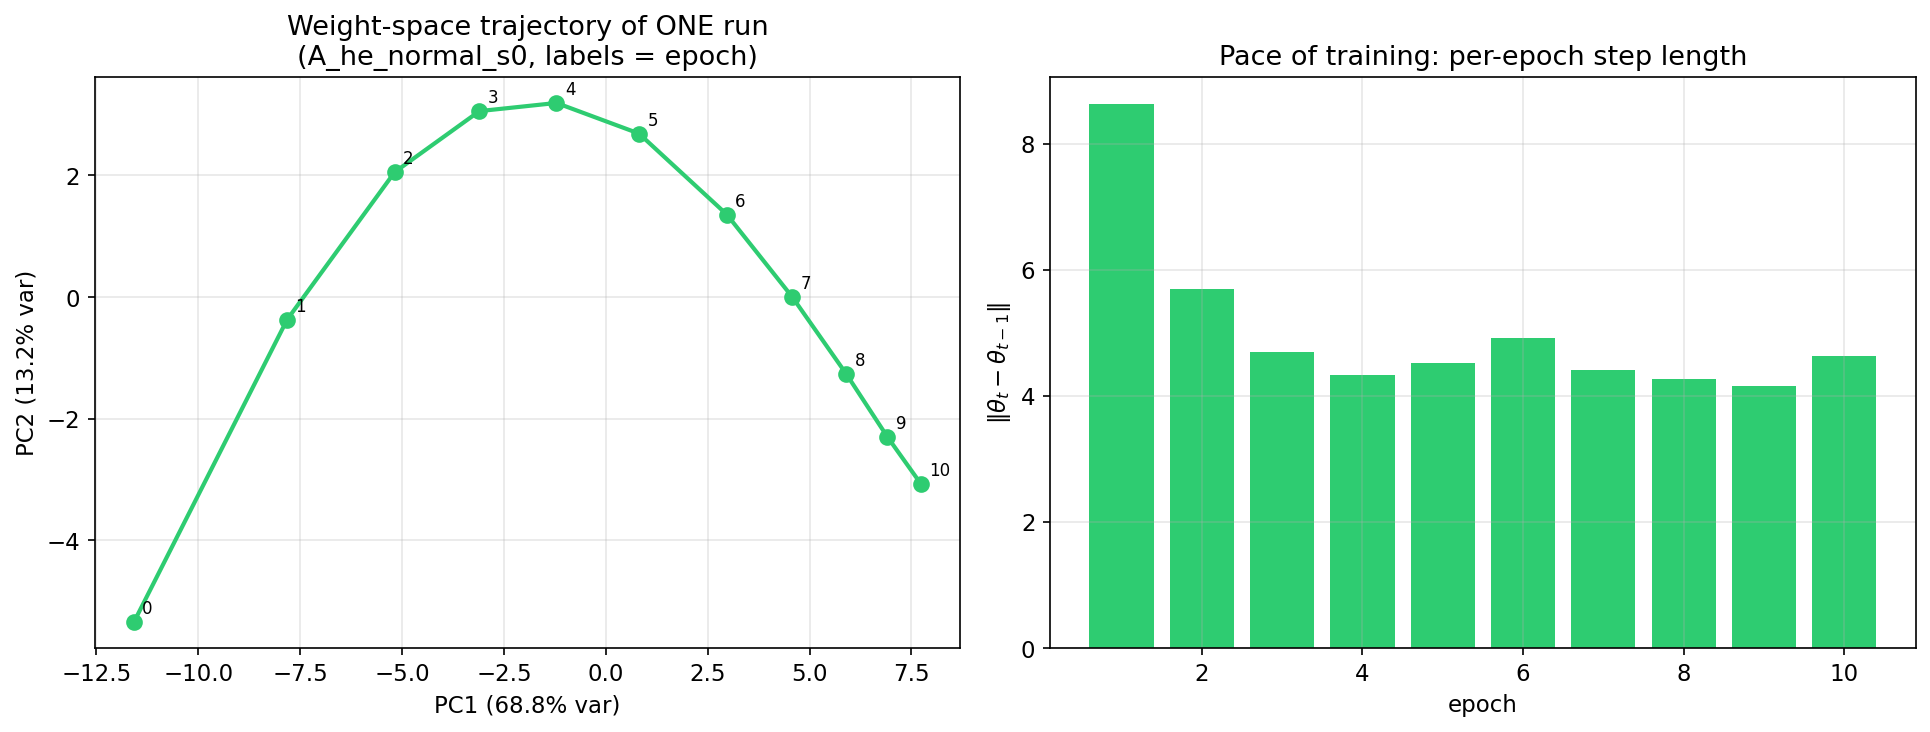
\includegraphics[width=\textwidth]{fig1_single_run_trajectory.png}
\caption{Weight-space trajectory of one run (\texttt{A\_he\_normal\_s0}, labels = epoch) and the
per-epoch step length. The path is monotone and the pace shows one large step, one intermediate,
then a plateau.}
\label{fig:traj}
\end{figure}

\textbf{That headline does not survive its null.} Table~\ref{tab:q1null} scores the same
statistics against a pure random walk with the identical step-size profile, and against the dead
run as a negative control.

\begin{table}[htbp]\centering
\caption{Q1 statistics against their nulls. $\mathrm{Spearman}=1.000$ is forced by $d\gg n$ and
carries no information. Straightness barely separates the dead run from the real one. Only the
consecutive-step cosine cleanly distinguishes learning from collapse.}
\label{tab:q1null}
\begin{tabular}{lcccc}
\toprule
Source & $\mathrm{EVR}_1$ & Spearman & Straightness & Step cosine \\
\midrule
Real run (\texttt{he\_normal}, 97.3\%)     & 0.689 & 1.000 & 0.400 & $+0.030$ \\
\textbf{Dead run} (\texttt{pytorch\_default}, 11.35\%) & 0.653 & 1.000 & 0.378 & $\mathbf{-0.146}$ \\
Random walk (mean of 200)                  & 0.578 & 1.000 & 0.326 & $-0.000$ \\
\bottomrule
\end{tabular}
\end{table}

$\mathrm{Spearman} = 1.000$ occurs in \textbf{100\% of 200 random-walk simulations}: with $n=11$
points in $d\approx5\times10^5$ dimensions it is geometrically forced. The dead network --- which
never learns --- also yields $\mathrm{EVR}_1 = 0.653$ and $\mathrm{Spearman} = 1.000$. Neither
statistic distinguishes learning from not learning. Straightness separates them only weakly
(0.400 vs 0.378). The one clean discriminator is the \textbf{consecutive-step cosine}: healthy
training has weak positive directional persistence ($+0.030$), while the dead network
\emph{anti}-aligns ($-0.146$), oscillating rather than advancing.

\begin{table}[htbp]\centering
\caption{Pace of training, single run. The first epoch carries 17.2\% of total distance and
almost all of the accuracy gain; the remaining nine cover 83\% of the distance for 3.4 further
points.}
\label{tab:pace}
\begin{tabular}{cccc|cccc}
\toprule
Epoch & Step & \% of total & Test acc (\%) & Epoch & Step & \% of total & Test acc (\%) \\
\midrule
1 & 8.627 & 17.2 & 93.92 & 6  & 4.922 & 9.8 & 96.22 \\
2 & 5.699 & 11.3 & 95.19 & 7  & 4.417 & 8.8 & 97.00 \\
3 & 4.694 &  9.3 & 95.94 & 8  & 4.263 & 8.5 & 97.19 \\
4 & 4.332 &  8.6 & 96.14 & 9  & 4.154 & 8.3 & 97.30 \\
5 & 4.526 &  9.0 & 96.30 & 10 & 4.626 & 9.2 & 97.31 \\
\bottomrule
\end{tabular}
\end{table}

The step-size profile (Table~\ref{tab:pace}) is the honest deliverable for ``pace'', and it is
genuinely interesting: \textbf{the network keeps moving at a near-constant rate long after the
functional gains stop}. Epoch~1 takes accuracy from 10.3\% to 93.9\%; the remaining nine epochs
travel five times as far in weight space for 3.4 further points. One caveat: with constant
learning rate and no scheduler, Adam's per-step displacement is only weakly tied to gradient
magnitude, so a plateau is partly expected --- the observed plateau (4.49) is $0.42\times$ the
free-running Adam bound $\text{lr}\sqrt{d}\sqrt{\text{steps}} = 10.82$.

\subsection{Q2 --- Initializations as starting points}

At depth 26 the schemes split cleanly into survivors and failures; at depth 10 every scheme
trains (Table~\ref{tab:acc}). Collapse is therefore a \emph{depth $\times$ initialization-scale
interaction}, not a property of the initialization alone.

\begin{table}[htbp]\centering
\caption{Final test accuracy by scheme and depth (mean of 3 seeds), with mean $|W|$ at epoch 0
from the 20-seed untrained population. The two schemes that fail at depth 26 are the two
smallest-magnitude initializations.}
\label{tab:acc}
\begin{tabular}{lccc c}
\toprule
Initialization & mean $|W|$ at ep.\ 0 & Depth 26 (\%) & Depth 10 (\%) & Survives depth 26 \\
\midrule
\texttt{pytorch\_default}    & 0.0432 & \textbf{11.35} & 97.39 & no \\
\texttt{lognormal\_jaynes}   & 0.0492 & \textbf{79.21} & 96.85 & degraded \\
\texttt{orthogonal}          & 0.0691 & 94.31 & 97.69 & yes \\
\texttt{xavier\_normal}      & 0.0702 & 96.77 & 97.68 & yes \\
\texttt{he\_normal}          & 0.0974 & 96.97 & 97.38 & yes \\
\texttt{lognormal\_he\_scale}& 0.0989 & 97.00 & 97.27 & yes \\
\texttt{he\_uniform}         & 0.1058 & 96.99 & 97.29 & yes \\
\bottomrule
\end{tabular}
\end{table}

\begin{figure}[htbp]\centering
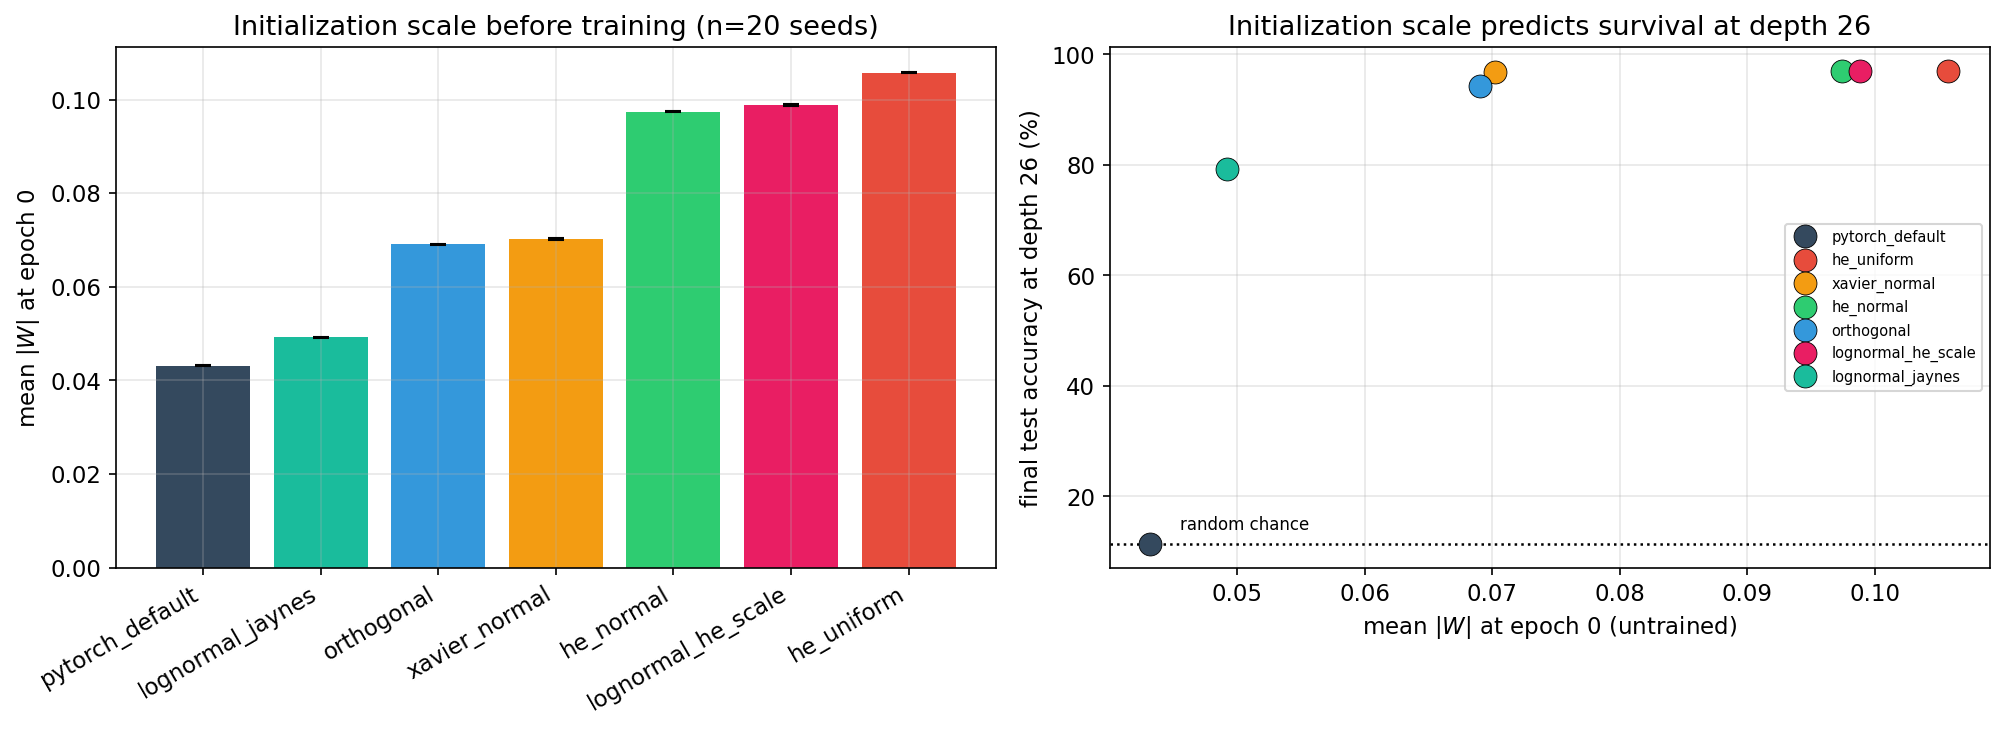
\includegraphics[width=\textwidth]{fig10_untrained_population.png}
\caption{The untrained population (20 seeds per scheme, epoch 0 only). Left: initialization scale
before any training, with seed-to-seed error bars far smaller than between-scheme differences.
Right: that scale against eventual survival at depth 26 --- the two failing schemes are the two
smallest-magnitude initializations.}
\label{fig:untrained}
\end{figure}

Initialization scale at epoch 0 rank-correlates with survival at depth 26 at
$\mathrm{Spearman} = +0.964$ ($n=7$). \textbf{The honest caveat is that this is close to true by
construction}: these schemes differ in weight variance by design, so separating them at epoch 0
largely restates their definitions. The defensible claim is the weaker one --- \emph{collapse is
determined by initialization scale} --- and the depth-10 control is what supports it. Notably,
\texttt{lognormal\_he\_scale} (log-normal at He variance) survives depth 26 at 97.0\% while
\texttt{lognormal\_jaynes} (log-normal at the Jaynes-paper parameters, but $2\times$ smaller
magnitude) degrades to 79.2\%: for log-normal initialization, \emph{scale matters more than
shape}.

\subsection{Q3 --- Is any initialization closer to the minima?}

All seven schemes fall in $D_{\text{norm}} \in [0.9995, 1.0006]$ (Table~\ref{tab:dnorm}). The
total between-scheme spread is $1.10\times10^{-3}$ against a measured null-draw noise floor of
$5.69\times10^{-4}$ --- the same order. The between-reference rank correlation is $+0.036$:
\textbf{there is no reproducible ranking at all}, and the ordering in Table~\ref{tab:dnorm}
should not be read.

\begin{table}[htbp]\centering
\caption{Distance from each initialization to a trained reference (\texttt{he\_normal\_s0},
epoch 10); \texttt{same\_run} and \texttt{same\_seed} pairs excluded. Ranking by raw
$d_{\text{aligned}}$ would crown \texttt{pytorch\_default} --- the dead scheme --- purely because
its weights are smallest.}
\label{tab:dnorm}
\begin{tabular}{lccccc}
\toprule
Initialization & $d_{\text{unaligned}}$ & $d_{\text{aligned}}$ & $d_{\text{null}}$ &
$D_{\text{norm}}$ & Norm gap \\
\midrule
\texttt{orthogonal}          &  99.89 &  90.14 &  90.18 & 0.9995 & 25.48 \\
\texttt{he\_normal}          & 114.84 & 102.84 & 102.89 & 0.9996 &  2.00 \\
\texttt{xavier\_normal}      & 100.36 &  90.66 &  90.66 & 1.0000 & 24.58 \\
\texttt{lognormal\_jaynes}   &  92.61 &  85.34 &  85.34 & 1.0000 & 39.40 \\
\texttt{he\_uniform}         & 114.74 & 102.87 & 102.85 & 1.0002 &  2.03 \\
\texttt{lognormal\_he\_scale}& 114.77 & 102.84 & 102.82 & 1.0002 &  2.04 \\
\texttt{pytorch\_default}    &  88.40 &  82.32 &  82.27 & 1.0006 & 49.29 \\
\bottomrule
\end{tabular}
\end{table}

\textbf{The null was load-bearing, not decorative.} Ranked by raw aligned distance the apparent
winner is \texttt{pytorch\_default}, \emph{the dead scheme}, because it simply has the smallest
weights: that ranking correlates with the norm gap at $\mathrm{Spearman} = -0.893$. Reporting raw
distance would have produced a confident and entirely spurious headline.

\subsubsection{Positive control: does the instrument fire at all?}

A null result is worthless without evidence the measurement could detect the effect. We
constructed initializations at known proximity,
$\theta_0 = \alpha\,\pi(\theta_T) + \sqrt{1-\alpha^2}\,\varepsilon$, and measured the response
(Table~\ref{tab:poscontrol}, Figure~\ref{fig:poscontrol}).

\begin{table}[htbp]\centering
\caption{$D_{\text{norm}}$ response at known overlap $\alpha$. The metric reaches 0 for a
permuted copy, so it is not pinned at 1 --- but it only departs from 1 above $\alpha\approx0.5$,
because below that the weight matcher recovers almost none of the true permutation.}
\label{tab:poscontrol}
\begin{tabular}{lccccccc}
\toprule
$\alpha$ & 0.0 & 0.1 & 0.2 & 0.3 & 0.5 & 0.7 & 1.0 \\
\midrule
$D_{\text{norm}}$        & 1.0007 & 0.9998 & 0.9987 & 0.9819 & \textbf{0.7856} & 0.6090 & \textbf{0.0000} \\
$\cos_{\text{aligned}}$  & 0.182  & 0.184  & 0.186  & 0.214  & 0.498  & 0.700  & 1.000 \\
\bottomrule
\end{tabular}
\end{table}

\begin{figure}[htbp]\centering
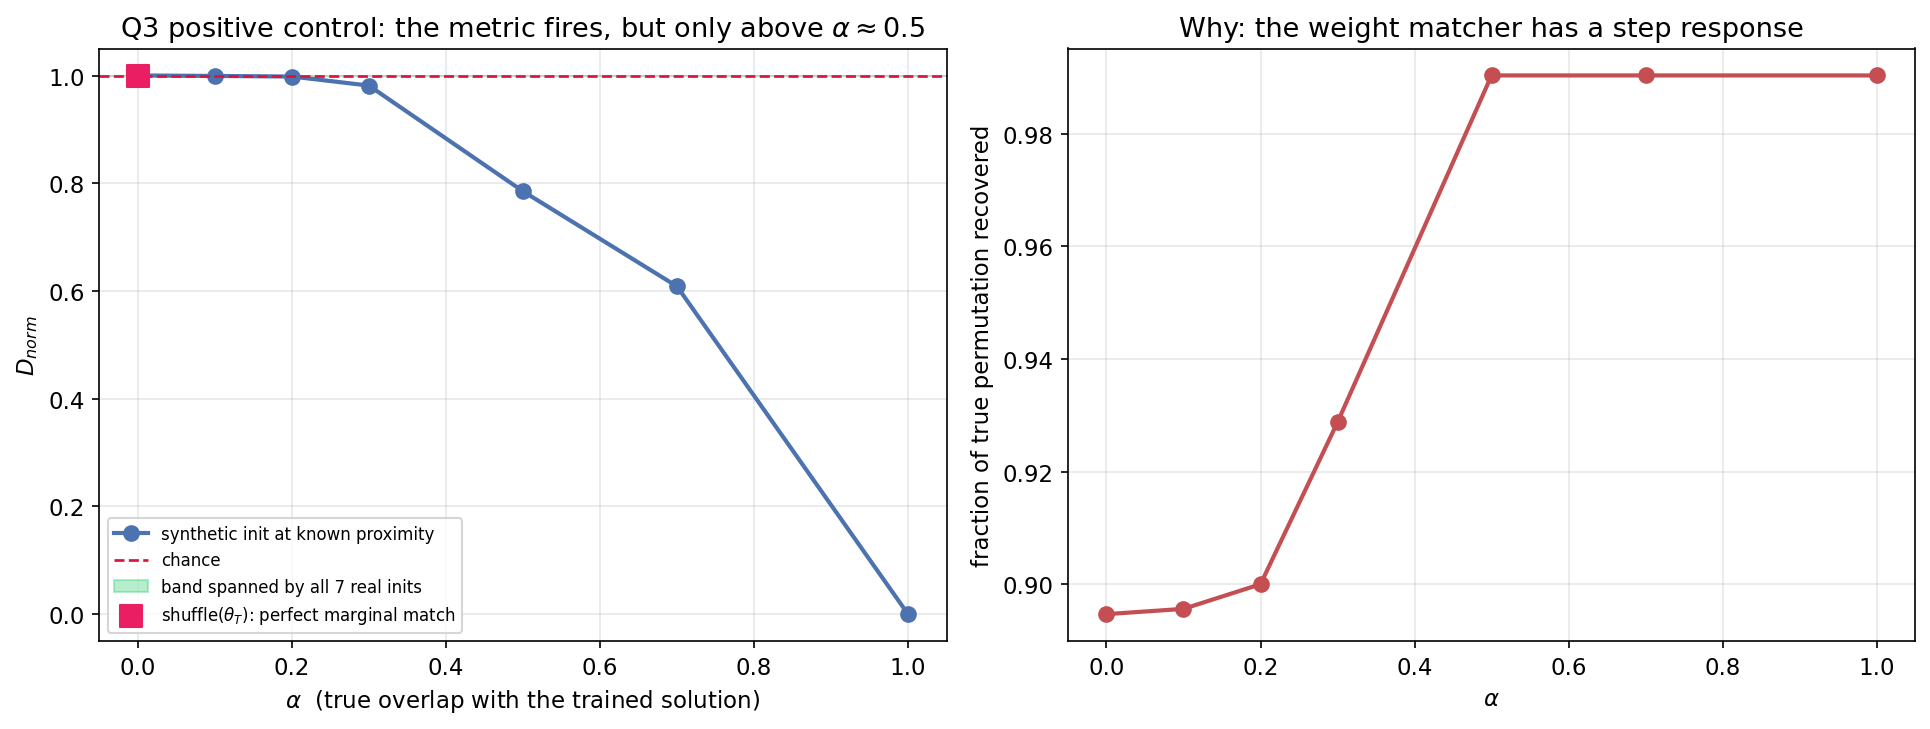
\includegraphics[width=\textwidth]{fig9_q3_positive_control.png}
\caption{Q3 calibration. Left: $D_{\text{norm}}$ against true overlap $\alpha$; the green band
spans all seven real schemes and the pink square is \texttt{shuffle}$(\theta_T)$. Right: the
weight matcher's step response explains why --- below $\alpha\approx0.5$ it recovers essentially
none of the true permutation.}
\label{fig:poscontrol}
\end{figure}

So the defensible statement is a \textbf{bound}, not an equality: \emph{no initialization reaches
post-alignment cosine $\gtrsim0.3$ with a trained solution} --- which no data-independent
initialization plausibly could.

\subsubsection{A limit this result does not overcome}

The null preserves every per-layer weight marginal by construction, so $D_{\text{norm}}$ is
\textbf{blind to distributional matching}. Empirically, \texttt{shuffle}$(\theta_T)$ --- a
\emph{perfect} per-layer distributional match to the trained network carrying zero neuron
structure --- scores $D_{\text{norm}} = 1.00019$, inside the band spanned by the real schemes.
\textbf{This result therefore does not test the log-normal hypothesis.} Testing that requires a
different null, and designing one is the natural next methodological step.

\subsection{When alignment matters: the cleanest result of the week}

Table~\ref{tab:drift} reports permutation drift by pair class. Within a single run, across
consecutive epochs, \textbf{0.0\% of neurons move} and alignment changes distance by
\textbf{0.00\%}. Across independently-seeded runs, 91.4\% of neurons move and alignment cuts
distance by 11.0\%.

\begin{table}[htbp]\centering
\caption{Permutation drift by pair class. SGD does not permute neurons mid-training.}
\label{tab:drift}
\begin{tabular}{lccc}
\toprule
Pair class & $n$ & Distance reduction from alignment & Fraction of neurons moved \\
\midrule
Consecutive epochs (same run)     & 60 & \textbf{0.00\%}  & \textbf{0.0000} \\
Trained models (different seeds)  & 21 & 10.99\%          & 0.9143 \\
\bottomrule
\end{tabular}
\end{table}

\begin{figure}[htbp]\centering
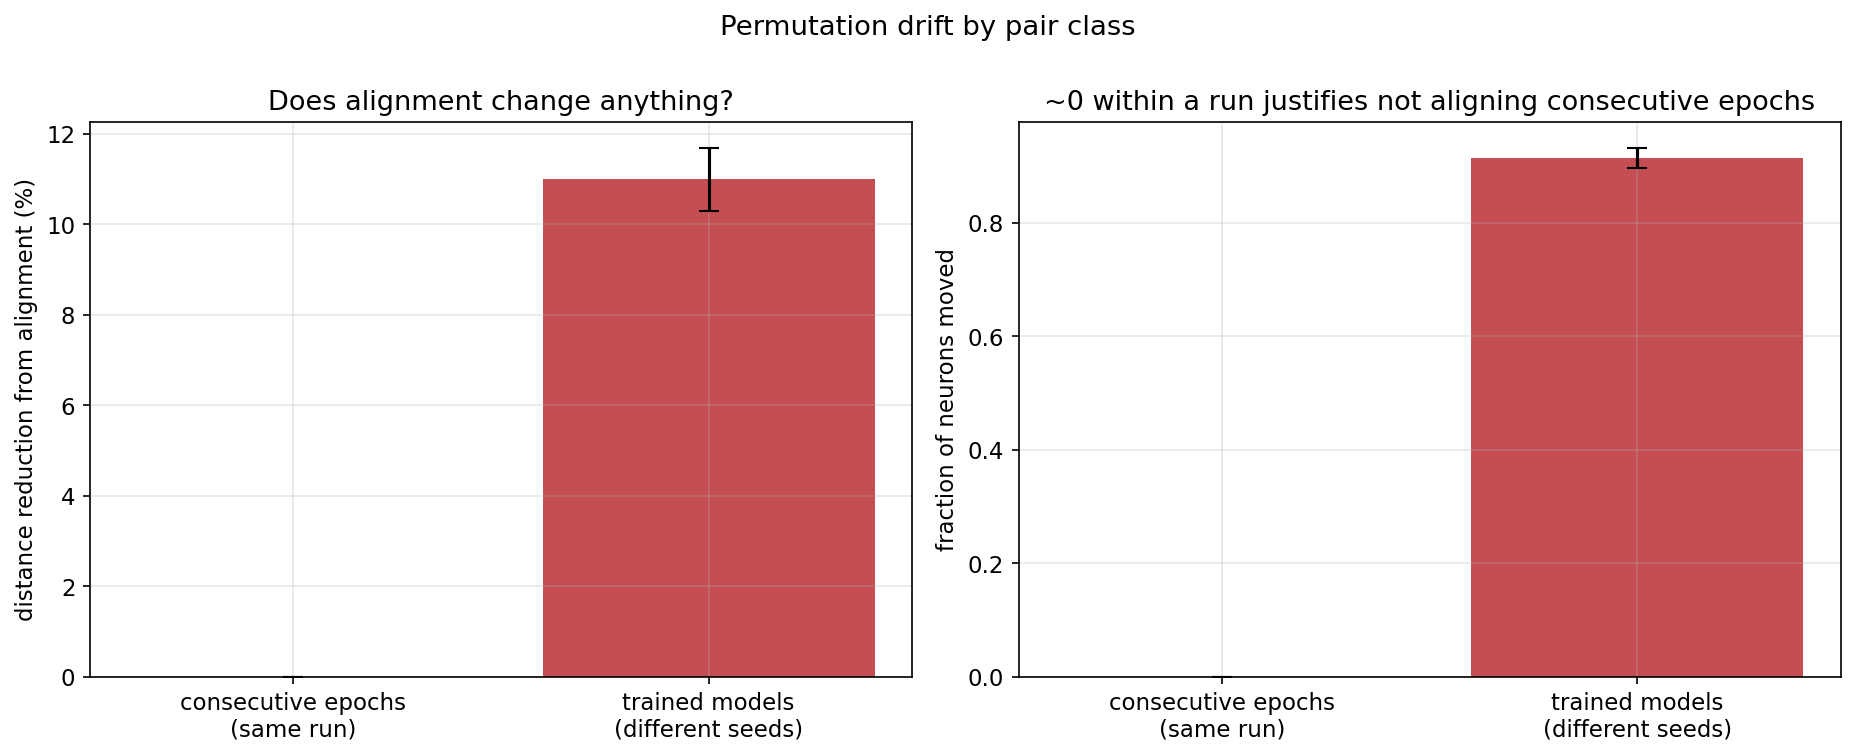
\includegraphics[width=0.92\textwidth]{fig7_alignment_necessity.png}
\caption{Permutation drift by pair class. Within a run alignment changes nothing (0.0\% of
neurons move); across independently-seeded runs it moves 91.4\% of neurons and cuts distance by
11.0\%.}
\label{fig:drift}
\end{figure}

This is not confounded by anything, and it has immediate practical consequence: \textbf{within-run
trajectories may be read directly without alignment, while any cross-run weight comparison is
meaningless without it.}

\subsection{A lead that was withdrawn}
\label{sec:withdrawn}

Spectral distance $D_{\text{spec}}$ from an initialization to a trained network initially appeared
to track final accuracy ($\mathrm{Spearman} = -0.857$), which would have been an attractive
finding. It does not survive scrutiny: $D_{\text{spec}}$ is rank-correlated $+0.929$ with the
plain norm gap and reproduces the norm gap's correlation with accuracy \emph{exactly}, while the
distributional $D_{\text{dist}}$ is rank-\emph{identical} to it ($+1.000$). Both are re-encodings
of weight scale rather than independent structural probes, so the ``lead'' is simply Q2 restated.

This also corrects a claim made earlier in the same analysis: since $\sigma(cW) = c\,\sigma(W)$
and $\log|cW| = \log|W| + \log c$, neither metric is scale-insensitive, and ReLU rescaling
remains genuinely unhandled.

\section{Discussion}

\subsection{What the nulls changed}

Three headline statistics were produced this week that would each have made a confident report
paragraph, and \emph{all three failed their nulls}:

\begin{enumerate}
\item $\mathrm{Spearman}(\mathrm{PC1},\mathrm{epoch}) = 1.000$ --- forced by $d\gg n$, and
reproduced by a network that never learns.
\item ``\texttt{pytorch\_default} starts closest to the minima'' --- an artifact of it having the
smallest weights.
\item ``Spectral distance predicts collapse'' --- a re-encoding of weight scale.
\end{enumerate}

In a $5\times10^5$-dimensional space with $n=11$ points per run and 7 schemes, statistics that
look decisive are frequently geometric inevitabilities. The practical lesson for the remainder of
this project is that \textbf{every weight-space statistic needs an explicit null and a positive
control before it is believed}, and that the positive control matters as much as the null --- a
metric pinned at chance is indistinguishable from a metric that cannot fire.

\subsection{Limitation: pooled weight-space PCA does not work}

Pooled across independently-seeded runs the absolute embedding is near-isotropic: the
explained-variance spectrum is flat ($0.153 / 0.152 / 0.139$), no direction dominates, and signed
PC1 correlates with nothing ($\rho\approx-0.001$ with weight norm) --- though since a PC's sign is
arbitrary, $|\mathrm{PC1}|$ does track scale ($\rho = +0.52$). Two different-seed initializations
have cosine $\approx-0.002$; in $\sim\!500{,}000$ dimensions independent random vectors are
essentially orthogonal, so no 2-D projection of the pooled cloud can be faithful.
\textbf{Weight-space PCA is a within-run instrument, or a displacement-space instrument --- not a
pooled one.} Converged solutions confirm this: they sit $90.3 \pm 10.9$ apart after alignment
(range 63.3--104.3), a broad cloud rather than a point.

\subsection{Relation to the project's central hypothesis}

The log-normal ``ideal state'' hypothesis is untouched by this week's Q3 result, for the reason
given in \S4.3.2. What the week does contribute is a sharper statement of what a successful
log-normal initialization would have to \emph{do}: since the minima form a broad cloud 90 units
wide and no data-independent initialization can reach cosine $\gtrsim0.3$ with any of them,
``initialize near the minimum'' is not an achievable target in weight space. The mechanism, if
one exists, must be about the \emph{trajectory} an initialization enables --- consistent with the
one place this week found real signal, the consecutive-step cosine.

There is also a concrete finding for log-normal initialization specifically:
\texttt{lognormal\_he\_scale} survives depth 26 at 97.0\% while \texttt{lognormal\_jaynes}
degrades to 79.2\%. The difference between them is variance, not distributional shape. Any future
log-normal initialization scheme should be parameterized by target variance, with the log-normal
shape as a secondary degree of freedom.

\section{Conclusion}

Treating the weight matrix as an embedding works, but is far more delicate than treating
activations as one, and most of this week's value came from the controls rather than the
measurements.

\begin{enumerate}
\item \textbf{Trajectory and pace (Q1): yes, with caveats.} The trajectory is real and the pace
is readable, but the natural summary statistics are geometric inevitabilities. What survives is
that healthy training has weak positive directional persistence ($+0.030$) while a collapsed
network anti-aligns ($-0.146$), and that the network continues moving at a near-constant rate long
after accuracy has plateaued.
\item \textbf{Starting points (Q2): separable, largely by construction.} Initialization scale
predicts survival at depth 26 ($\rho = +0.964$), but these schemes differ in scale by design. For
log-normal specifically, scale matters more than shape.
\item \textbf{Optimal init near the minima (Q3): a bound, not an equality.} All schemes are
indistinguishable within noise; the instrument is calibrated and fires above $\alpha\approx0.5$;
and the null is blind to distributional matching, so this does not bear on the log-normal
hypothesis.
\item \textbf{Methodological (strongest result):} SGD does not permute neurons mid-training
(0.0\% vs 91.4\% across seeds). Within-run trajectories can be read directly; cross-run
comparisons cannot be made without alignment.
\end{enumerate}

\subsection*{Next step}

The non-trivial version of Q2 --- \emph{does seed-level position at epoch 0 predict survival
within a single scheme?} --- cannot be answered by restating an initialization formula. It
requires a configuration sitting exactly on the collapse boundary, swept over many seeds so that
some runs live and some die under an identical scheme. Week~16's boundary (depth 30, width 512,
with BatchNorm, which oscillated between 55\% and 96\%) is the natural candidate. Alongside it,
a null that is \emph{not} blind to marginal distribution would let Q3 finally speak to the
log-normal hypothesis directly.

\appendix
\section{Why \texttt{weight\_decay} = 0}

Same dead network, same seed, only weight decay changes:

\begin{table}[htbp]\centering
\begin{tabular}{lccccc}
\toprule
Weight decay & Test acc (\%) & mean $|W|$ ep.\ 0 & mean $|W|$ ep.\ 10 & Change & Log-normal $R^2$ \\
\midrule
$0$        & 11.35 & 0.04324 & 0.04316 & $0.998\times$ & 0.818 \\
$10^{-4}$  & 11.35 & 0.04324 & 0.00049 & $\mathbf{0.011\times}$ & 0.914 \\
\bottomrule
\end{tabular}
\end{table}

Both rows are the same dead network at identical accuracy. With $\text{wd}=0$ its weights stay
where they were initialized; with $\text{wd}=10^{-4}$ they are shrunk $89\times$ toward zero,
because a dead network receives essentially no gradient and decay acts unopposed. Since this week
measures distance between parameter vectors, that pull would bias every number --- hence
$\text{wd}=0$ throughout.

Incidentally this reproduces the ``log-normal paradox'' noted in Week~18: the collapsed network
fits a log-normal distribution \emph{better} ($R^2 = 0.914$ vs $0.818$) precisely because its
weights have been crushed into a narrow, near-zero distribution. Log-normal fit quality alone is
not evidence of a healthy state.

\section*{Reproducibility}

All results are produced by a single self-contained notebook,
\texttt{week1\_weight\_space\_trajectory.ipynb}, in \texttt{Fall\_26/Week 1/}. Every figure is
written alongside a \texttt{\_points.csv} containing its exact plotted values, indexed by
\texttt{MANIFEST.csv}. Training is resume-safe: with snapshots present the notebook skips
straight to analysis ($\approx$3~min); from scratch the full sweep takes $\approx$25~min on CPU.

\begin{thebibliography}{9}
\bibitem{ainsworth} Samuel K. Ainsworth, Jonathan Hayase, and Siddhartha Srinivasa.
Git Re-Basin: Merging models modulo permutation symmetries. \emph{arXiv:2209.04836}, 2022.
\bibitem{li} Hao Li, Zheng Xu, Gavin Taylor, Christoph Studer, and Tom Goldstein.
Visualizing the loss landscape of neural nets. \emph{NeurIPS}, 2018.
\bibitem{venkat} Venkat Venkatasubramanian, N. Sanjeevrajan, and Manasi Khandekar.
Jaynes machine: The universal microstructure of deep neural networks.
\emph{arXiv:2310.06960}, 2023.
\bibitem{uzan} Herut Uzan, Shira Sardi, Amir Goldental, and Ido Kanter. Stationary log-normal
distribution of weights stems from spontaneous ordering in adaptive node networks.
\emph{Physical Review E}, 100(5):052303, 2019.
\end{thebibliography}

\end{document}
